\begin{minipage}{0.5\linewidth}

\section{Risse}


	\textbf{Ursachen}:
	\begin{itemize}
		\item zu rasches Austrocknen
		\item Temperatureinwirkungen
		\item Schwinden
		\item Lasteinwirkung
		\item Aufgezwungene oder behinderte Verformung
		\item Frosteinwirkung
		
	\end{itemize}

	\textbf{Anforderungen}
\begin{itemize}
	\item Normale Anforderungen: bei Erreichen von f$_{ctd}$: $ \sigma_s \leq f_{sd} \rightarrow $  sprödes Versagen verhindern (Mindestbewehrung) \& aufgezwungene und behindernde Verformungen begrenzen
	
%	\item Erhöhte Anforderungen (gute Rissverteiung): $ \sigma_s \leq f_{sd} \rightarrow $ Mindestbewehrung \& $ \sigma_s \leq f_{sd} -80 N/mm^2 \rightarrow $ Fliessen der Bewehrung häufiger Lastfälle verhindern \& $ \sigma_s \leq \sigma_{s,adm} \rightarrow $ um Rissbreiten (w$_{nom}$ = 0.5 mm) aufgezwungener und behinderter Verformungen oder qs Lasten begrenzen
%	
%	\item Hohe Anforderungen (Rissbreitenbegrenzung für ständige \& qs Lastfälle): $ \sigma_s \leq f_{sd} \rightarrow $ Mindestbewehrung \& $\sigma_s \leq f_{sd} - 80 N/mm^2 \rightarrow $ Fliessen der Bewehrung häufiger Lastfälle verhindern \& $ \sigma_s \leq \sigma_{s,adm} \rightarrow $ um Rissbreiten (w$_{nom}$ = 0.2 mm) aufgezwungener und behinderter Verformungen oder qs Lasten begrenzen
	
\end{itemize}

\end{minipage}
\begin{minipage}{0.5\linewidth}
%	\textbf{Anforderungen}
		\begin{itemize}
%			\item Normale Anforderungen: bei Erreichen von f$_{ctd}$: $ \sigma_s \leq f_{sd} \rightarrow $  sprödes Versagen verhindern (Mindestbewehrung) \& aufgezwungene und behindernde Verformungen begrenzen
		
			\item Erhöhte Anforderungen (gute Rissverteiung): $ \sigma_s \leq f_{sd} \rightarrow $ Mindestbewehrung \& $ \sigma_s \leq f_{sd} -80 N/mm^2 \rightarrow $ Fliessen der Bewehrung häufiger Lastfälle verhindern \& $ \sigma_s \leq \sigma_{s,adm} \rightarrow $ um Rissbreiten (w$_{nom}$ = 0.5 mm) aufgezwungener und behinderter Verformungen oder qs Lasten begrenzen
		
			\item Hohe Anforderungen (Rissbreitenbegrenzung für ständige \& qs Lastfälle): $ \sigma_s \leq f_{sd} \rightarrow $ Mindestbewehrung \& $\sigma_s \leq f_{sd} - 80 N/mm^2 \rightarrow $ Fliessen der Bewehrung häufiger Lastfälle verhindern \& $ \sigma_s \leq \sigma_{s,adm} \rightarrow $ um Rissbreiten (w$_{nom}$ = 0.2 mm) aufgezwungener und behinderter Verformungen oder qs Lasten begrenzen
			
		\end{itemize}
\end{minipage}





\begin{minipage}{0.8\linewidth}
	
	\subsection{Zugelement}
	
		\begin{tabular}{l|p{0.3\linewidth}|l}
			
			Bemerkung		& Formel		& Einheit \\ \hline
			
			
			Bewehrungsquerschnitt	&	$ A_s = n_s \cdot \pi \cdot \frac{\oslash^2}{4} $	& [mm] \\
		
			Bewehrungsgehalt		&	$ \rho = \frac{A_s}{A} $ &  \\
			
			Betonquerschnitt		&	$ A_c =  A - A_s = A \cdot (1 - \rho) $ &	[mm]	\\
			
			Querschnittsbeiwert		&	$ n = \alpha = \frac{E_s}{E_c} $	&	\\
			Ideellerquerschnitt		& $ A_i = (A - A_s) + n \cdot A_s = A_c + n \cdot A_s = A \cdot (1 + \rho \cdot (n - 1)) $	& [mm]	\\
			
			Rissbreite				&	$ w = \int (\varepsilon_s - \varepsilon_c) dx \approx \frac{\oslash}{8 \cdot \rho} \frac{f_{ct}}{E_s} $	& [mm] \\
%			$ \rightarrow $ mit $ \rho = \frac{f_{ct}}{\sigma_s^{\rom{2}}} $	& $ w = \frac{\oslash}{8} \frac{\sigma_s^{\rom{2} \cdot 2}}{f_{ct} \cdot E_s} $	& [mm] \\
			$ \rightarrow $ mit $ \rho = \frac{f_{ct}}{\sigma_s^\amalg} $	& $ w = \frac{\oslash}{8} \frac{\sigma_s^{\amalg \cdot 2}}{f_{ct} \cdot E_s} $	& [mm] \\
									& $ \Rightarrow \sigma_s = \sqrt{ \frac{8 \cdot f_{ck} \cdot E_s \cdot w}{\oslash}} $ &	$ \left[ \frac{kN}{mm^2}\right]$ \\
									
			Rissabstand				&	$ 1 l_b \leq S_r \leq 2 l_b $  & 	[mm] \\
			
			Risslast				&	$ N_r = f_{ct} \cdot A_i $	& [kN] \\
			$ \rightarrow $ erf. A$_{s,min} $ &	&	\\
%			$ \rightarrow $ erf. A$_{s,min} $ & $ \rightarrow $ je höher f$_{ck}$ (f$_{ct}$), desto höher A$_{s,min}$ (A$_{s,Riss}$) 	&	\\
%									& Rissbildung an der schwächsten Stelle & \\
%									& $ \rightarrow $ mehr Bewehrung $ \Rightarrow $ kleienr l$_b$, kleiner w, mehr kleine Risse pro Meter & \\
%									& grosse $ \oslash $ weniger effektiv $ \rightarrow $ gr. Rissbreite & \\
												
		\end{tabular}
\end{minipage}
\begin{minipage}{0.2\linewidth}
		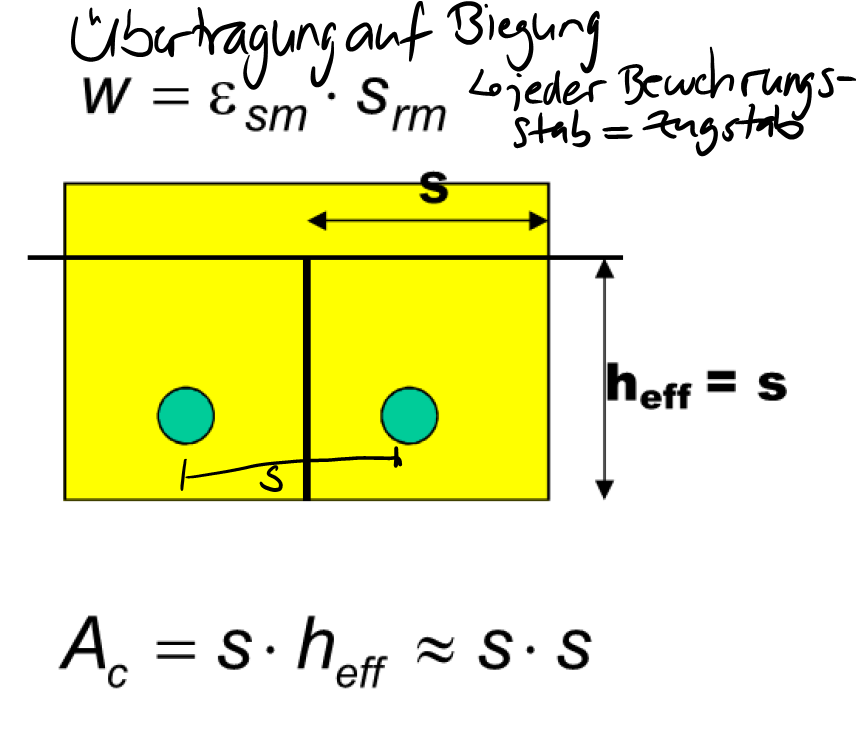
\includegraphics[width=\linewidth]{images/Risse1Zugelement.PNG}
		$ \rightarrow $ je höher f$_{ck}$ (f$_{ct}$), desto höher A$_{s,min}$ (A$_{s,Riss}$) \\
		Rissbildung an der schwächsten Stelle \\
		$ \rightarrow $ mehr Bewehrung $ \Rightarrow $ kleienr l$_b$, kleiner w, mehr kleine Risse pro Meter \\
		grosse $ \oslash $ weniger effektiv $ \rightarrow $ gr. Rissbreite \\	
\end{minipage}







%\begin{minipage}{0.8\linewidth}
%	
%	\subsection{Querschnittsanalysen, reine Biegung}
%	
%	\subsubsection{Rechteckquerschnitt ohne Druckbewehrung}
%	
%	
%		\begin{tabular}{p{0.3\linewidth}|l|l}
%			
%		Bemerkung		& Formel		& Einheit \\ \hline
%		
%		
%		Spannungsberechnung	& $ E_{cm\infty} = \frac{E_{cm,0}}{1 + \varphi} $ und $ n = \frac{E_s}{E_{cm\infty}} $	& $ \left[ \frac{kN}{mm^2}\right] $ \\
%		
%		Statisches Moment	& $ S_i = 0 = 
%							\textcolor{red}{ b \cdot x \cdot \frac{x}{2} } - 
%							\textcolor{blue}{ (d - x) \cdot n \cdot A_s } $ & [mm$^3$] \\
%		S$_i$ der ideellen Fläche muss bez. der neutralen Achse Null sein &	& \\
%		
%		Druckzonenhöhe		& $ x = n \cdot \frac{A_s}{b} \left( \sqrt{1 + \frac{2 b d}{n A_s}} - 1 \right) $ & [mm] \\
%		$ \rightarrow $ aus Bedigung S$_i$=0 & & \\
%		
%		Flächenmoment		& $ I_{Rechteck,i} = \frac{b \cdot x^3}{3} + n A_s (d - x)^2 $	& [mm$^4$] \\
%		
%		Verträglichkeitsbedingung & $ \frac{\varepsilon_s}{\varepsilon_c} = \frac{d - x}{x}
%		\Rightarrow \varepsilon_s = \frac{d - x}{x} \varepsilon_c $	& \\
%								 & $ E_s \cdot \varepsilon_s = \sigma_s = E_s \cdot \varepsilon_c \frac{d - x}{x} = n \cdot \sigma_c \frac{d - x}{x} $	& $ \left[ \frac{kN}{mm^2}\right] $ 	\\
%								 
%		Stahlspannung			& $ \sigma_s = n \frac{M}{I_i} (d - x) $	& $ \left[ \frac{kN}{mm^2}\right] $ \\
%								& $ \sigma_s = \frac{M}{0.9 \cdot d \cdot A_s} $	& \\
%			
%		\end{tabular}
%\end{minipage}
%\begin{minipage}{0.3\linewidth}
%	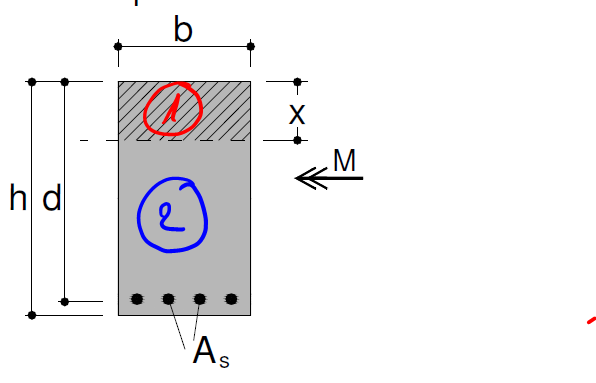
\includegraphics[width=\linewidth]{images/Risse2QSRechtecko.PNG}
%\end{minipage}
%
%
%
%
%
%
%\begin{minipage}{0.8\linewidth}
%	
%	\subsubsection{Rechteckquerschnitt mit Druckbewehrung}
%	
%	
%	\begin{tabular}{p{0.3\linewidth}|l|l}
%		
%		Bemerkung		& Formel		& Einheit \\ \hline
%		
%		
%		Spannungsberechnung	& $ E_{cm\infty} = \frac{E_{cm,0}}{1 + \varphi} $ und $ n = \frac{E_s}{E_{cm\infty}} $	& $ \left[ \frac{kN}{mm^2}\right] $ \\
%		
%		Statisches Moment	& $ S_i = 0 = b \cdot x \cdot \frac{x}{2} + n \cdot A_s' (x - d') - (d - x) \cdot n \cdot A_s $ & [mm$^3$] \\
%		S$_i$ der ideellen Fläche muss bez. der neutralen Achse Null sein &	& \\
%		
%		Druckzonenhöhe		& $ x = n \cdot \frac{A_s + A_s'}{b} \left( \sqrt{1 + \frac{2 b d}{n} \frac{A_s + A_s' \frac{d'}{d}}{(A_s + A_s')^2} } - 1 \right) $ & [mm] \\
%		$ \rightarrow $ aus Bedigung S$_i$=0 & & \\
%		
%		Flächenmoment		& $ I_{Rechteck,i} = \frac{b \cdot x^3}{3} + n \cdot A_s' (x - d')^2 + n \cdot A_s (d - x)^2 $	& [mm$^4$] \\
%		
%		Verträglichkeitsbedingung & $ \frac{\varepsilon_s}{\varepsilon_c} = \frac{d - x}{x}
%		\Rightarrow \varepsilon_s = \frac{d - x}{x} \varepsilon_c $	& \\
%		& $ E_s \cdot \varepsilon_s = \sigma_s = E_s \cdot \varepsilon_c \frac{d - x}{x} = n \cdot \sigma_c \frac{d - x}{x} $	& $ \left[ \frac{kN}{mm^2}\right] $ 	\\
%		
%		Stahlspannung			& $ \sigma_s = n \frac{M}{I_i} (d - x) $	& $ \left[ \frac{kN}{mm^2}\right] $ \\
%		
%	\end{tabular}
%\end{minipage}
%\begin{minipage}{0.3\linewidth}
%	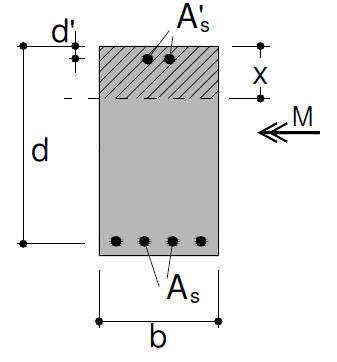
\includegraphics[width=\linewidth]{images/Risse3QSRechteckm.PNG}
%\end{minipage}
%
%
%
%
%\subsubsection{Plattenbalkenquerschnitt}
%
%\begin{minipage}{0.8\linewidth}
%	\begin{tabular}{p{0.3\linewidth}|p{0.5\linewidth}|l}
%		
%		Bemerkung		& Formel		& Einheit \\ \hline
%		
%		
%		abklären ob x $ \leq $ h$_f$ oder x > h$_f$ & & \\
%		
%						& $ S_i (x = h_f) =  b \cdot \frac{h_f^2}{2} + n \cdot A_s' (h_f - d') - n \cdot A_s (d - h_f)  $ & [mm$^3$] \\
%		\textcolor{red}{1} S$_i$ (x = h$_f$) > 0 $ \rightarrow $ Berechnen am Rechteck QS &	& \\
%		\textcolor{red}{2} S$_i$ (x = h$_f$) < 0 $ \rightarrow $ Berechnen am Plattenbalken QS (Druck bis in Steg) &	& \\
%		
%		falls Plattenbalken: Statisches Moment	& $ S_i = 0 = (b - b_w) h_f \left( x - \frac{h_f}{2} \right) + \frac{b_w \cdot x^2}{2} + n \cdot A_s' (x - d') - n \cdot A_s (d - x) \rightarrow x $	&  [mm$^3$] \\
%		
%		Flächenmoment		& $ I_{i} = (b - b_w) \frac{h_f^3}{12} + (b - b_w) h_f \left( x - \frac{h_f}{2} \right)^2 + \frac{b_w \cdot x^3}{3} + n \cdot A_s' (x - d')^2 + n \cdot A_s (d - x)^2 $	& [mm$^4$] \\
%		
%		Verträglichkeitsbedingung & $ \frac{\varepsilon_s}{\varepsilon_c} = \frac{d - x}{x}
%		\Rightarrow \varepsilon_s = \frac{d - x}{x} \varepsilon_c $	& \\
%		& $ E_s \cdot \varepsilon_s = \sigma_s = E_s \cdot \varepsilon_c \frac{d - x}{x} = n \cdot \sigma_c \frac{d - x}{x} $	& $ \left[ \frac{kN}{mm^2}\right] $ 	\\
%		
%		Stahlspannung			& $ \sigma_s = n \frac{M}{I_i} (d - x) $	& $ \left[ \frac{kN}{mm^2}\right] $ \\
%		
%	\end{tabular}
%\end{minipage}
%\begin{minipage}{0.3\linewidth}
%	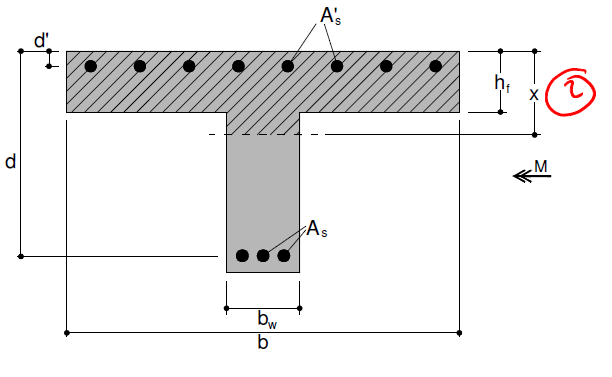
\includegraphics[width=\linewidth]{images/Risse4Plattenbalken.PNG}
%\end{minipage}




\begin{landscape}
	
	\begin{multicols}{3}
		
		
		\subsection{Querschnittsanalysen, reine Biegung}
		
		\subsubsection{Rechteckquerschnitt ohne Druckbewehrung}
		
		
		\begin{tabular}{p{0.4\linewidth}|p{0.4\linewidth}|l}
			
			Bemerkung		& Formel		& Einheit \\ \hline
			
			
			\hspace*{0pt} Spannungsberechnung	& $ E_{cm\infty} = \frac{E_{cm,0}}{1 + \varphi} $ und $ n = \frac{E_s}{E_{cm\infty}} $	& $ \left[ \frac{kN}{mm^2}\right] $ \\
			
			Statisches Moment	& $ S_i = 0 = 
			\textcolor{red}{ b \cdot x \cdot \frac{x}{2} } - 
			\textcolor{blue}{ (d - x) \cdot n \cdot A_s } $ & [mm$^3$] \\
			S$_i$ der ideellen Fläche muss bez. der neutralen Achse Null sein &	& \\
			
			Druckzonenhöhe		& $ x = n \cdot \frac{A_s}{b} \left( \sqrt{1 + \frac{2 b d}{n A_s}} - 1 \right) $ & [mm] \\
			$ \rightarrow $ aus Bedigung S$_i$=0 & & \\
			
			Flächenmoment		& $ I_{Rechteck,i} = \frac{b \cdot x^3}{3} + n A_s (d - x)^2 $	& [mm$^4$] \\
			
			\hspace*{0pt} Verträglichkeitsbedingung & $ \frac{\varepsilon_s}{\varepsilon_c} = \frac{d - x}{x}
			\Rightarrow \varepsilon_s = \frac{d - x}{x} \varepsilon_c $	& \\
			& $ E_s \cdot \varepsilon_s = \sigma_s = E_s \cdot \varepsilon_c \frac{d - x}{x} = n \cdot \sigma_c \frac{d - x}{x} $	& $ \left[ \frac{kN}{mm^2}\right] $ 	\\
			
			Stahlspannung			& $ \sigma_s = n \frac{M}{I_i} (d - x) $	& $ \left[ \frac{kN}{mm^2}\right] $ \\
			& $ \sigma_s = \frac{M}{0.9 \cdot d \cdot A_s} $	& \\
			
		\end{tabular}
		
		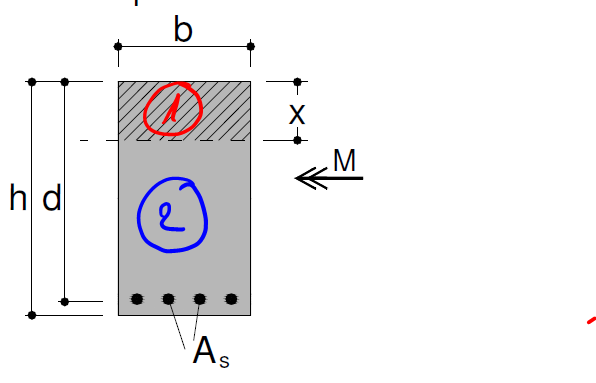
\includegraphics[width=0.6\linewidth]{images/Risse2QSRechtecko.PNG}
		
		
		
		
		
		\subsubsection{Rechteckquerschnitt mit Druckbewehrung}
		
		
		\begin{tabular}{p{0.4\linewidth}|p{0.4\linewidth}}
			
			Bemerkung		& Formel	 \\ \hline
			
			
			\hspace*{0pt} Spannungsberechnung	& $ E_{cm\infty} = \frac{E_{cm,0}}{1 + \varphi} $ und $ n = \frac{E_s}{E_{cm\infty}} $  \\
			
			Statisches Moment	& $ S_i = 0 = b \cdot x \cdot \frac{x}{2} + n \cdot A_s' (x - d') - (d - x) \cdot n \cdot A_s $  \\
			S$_i$ der ideellen Fläche muss bez. der neutralen Achse Null sein &	 \\
			
			Druckzonenhöhe		& $ x = n \cdot \frac{A_s + A_s'}{b} \left( \sqrt{1 + \frac{2 b d}{n} \frac{A_s + A_s' \frac{d'}{d}}{(A_s + A_s')^2} } - 1 \right) $   \\
			$ \rightarrow $ aus Bedigung S$_i$=0 &  \\
			
			Flächenmoment		& $ I_{Rechteck,i} = \frac{b \cdot x^3}{3} + n \cdot A_s' (x - d')^2 + n \cdot A_s (d - x)^2 $	  \\
			
			\hspace*{0pt} Verträglichkeitsbedingung & $ \frac{\varepsilon_s}{\varepsilon_c} = \frac{d - x}{x}
			\Rightarrow \varepsilon_s = \frac{d - x}{x} \varepsilon_c $	 \\
			& $ E_s \cdot \varepsilon_s = \sigma_s = E_s \cdot \varepsilon_c \frac{d - x}{x} = n \cdot \sigma_c \frac{d - x}{x} $		\\
			
			Stahlspannung			& $ \sigma_s = n \frac{M}{I_i} (d - x) $	 \\
			
		\end{tabular}
		
		
		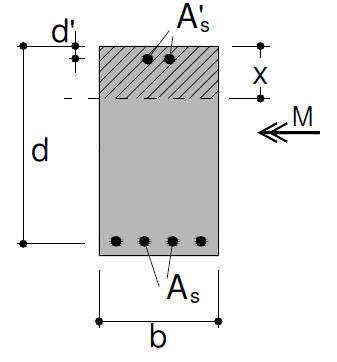
\includegraphics[width=0.4\linewidth]{images/Risse3QSRechteckm.PNG}
		
		
		
		
		
		\subsubsection{Plattenbalkenquerschnitt}
		
		
		\begin{tabular}{p{0.4\linewidth}|p{0.6\linewidth}}
			
			Bemerkung		& Formel	 \\ \hline
			
			
			abklären ob x $ \leq $ h$_f$ oder x > h$_f$ & \\
			
			& $ S_i (x = h_f) =  b \cdot \frac{h_f^2}{2} + n \cdot A_s' (h_f - d') - n \cdot A_s (d - h_f)  $   \\
			\textcolor{red}{1} S$_i$ (x = h$_f$) > 0 $ \rightarrow $ Berechnen am Rechteck QS &	 \\
			\textcolor{red}{2} S$_i$ (x = h$_f$) < 0 $ \rightarrow $ Berechnen am Plattenbalken QS (Druck bis in Steg) &	 \\
			
			falls Plattenbalken: Statisches Moment	& $ S_i = 0 = (b - b_w) h_f \left( x - \frac{h_f}{2} \right) + \frac{b_w \cdot x^2}{2} + n \cdot A_s' (x - d') - n \cdot A_s (d - x) \rightarrow x $  \\
			
			Flächenmoment		& $ I_{i} = (b - b_w) \frac{h_f^3}{12} + (b - b_w) h_f \left( x - \frac{h_f}{2} \right)^2 + \frac{b_w \cdot x^3}{3} + n \cdot A_s' (x - d')^2 + n \cdot A_s (d - x)^2 $	  \\
			
			\hspace*{0pt} Verträglichkeitsbedingung & $ \frac{\varepsilon_s}{\varepsilon_c} = \frac{d - x}{x}
			\Rightarrow \varepsilon_s = \frac{d - x}{x} \varepsilon_c $	 \\
			& $ E_s \cdot \varepsilon_s = \sigma_s = E_s \cdot \varepsilon_c \frac{d - x}{x} = n \cdot \sigma_c \frac{d - x}{x} $		\\
			
			Stahlspannung			& $ \sigma_s = n \frac{M}{I_i} (d - x) $ \\
			
		\end{tabular}
		
		
		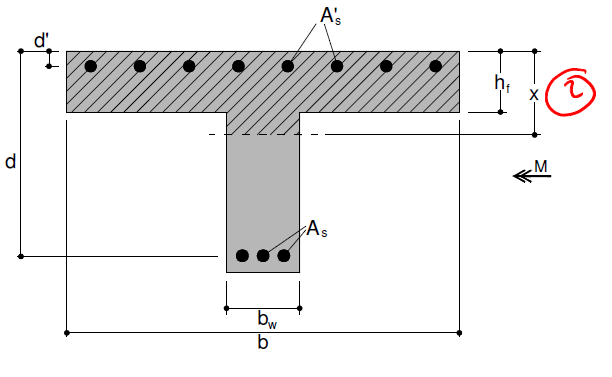
\includegraphics[width=0.7\linewidth]{images/Risse4Plattenbalken.PNG}
		
		
	\end{multicols}
	
\end{landscape}



%\subsection{Biegung mit Normalkraft}
%
%\begin{minipage}{0.35\linewidth}
%	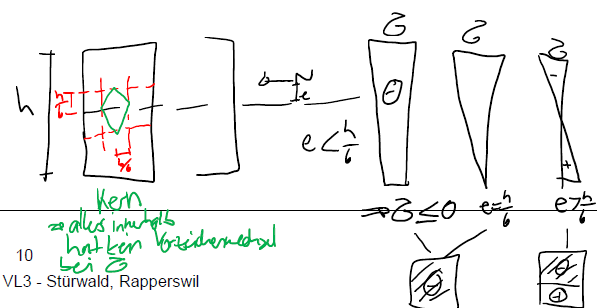
\includegraphics[width=0.8\linewidth]{images/Risse6Kern.PNG}
%\end{minipage}
%\begin{minipage}{0.6\linewidth}
%	Kernweiten:	 $ k_{1/2} = \frac{I_i}{A_i \cdot y_{2/1}} = \frac{W_y}{A} = \frac{  \frac{b \cdot h^2}{6}  }{b \cdot h} $  [m] \\
%	
%	Exzentrizität: $ e = -\frac{M}{N} $ [mm] \\
%\end{minipage}
%
%
%\subsubsection{Druck, kleine Exzentrizität}
%
%\begin{minipage}{0.35\linewidth}
%	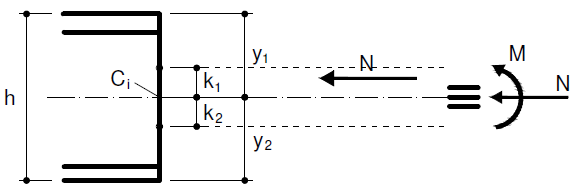
\includegraphics[width=0.8\linewidth]{images/Risse5klExPNG}
%	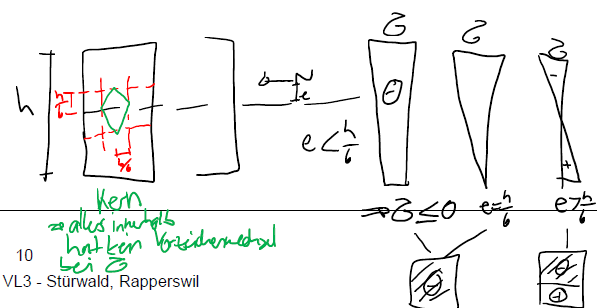
\includegraphics[width=0.8\linewidth]{images/Risse6Kern.PNG}
%\end{minipage}
%\begin{minipage}{0.6\linewidth}
%
%Greift N im Kern an, kann die Ausmitte vernachlässigt werden $ \rightarrow $ zentrischer Druck
%
%	\begin{tabular}{p{0.3\linewidth}|p{0.3\linewidth}|l}
%		
%		Bemerkung		& Formel		& Einheit \\ \hline
%		
%	
%		Spannung		& $ \sigma_c = \varepsilon_c \cdot E_c = \frac{N}{A_i} \pm \frac{M}{I_i}y $	& $ \left[ \frac{kN}{mm^2} \right]$ \\
%						& $ \sigma_s = \varepsilon_s \cdot E_s = n \cdot \sigma_c $	& $ \left[ \frac{kN}{mm^2} \right]$ \\
%		 
%		 Steifigkeit	& $ EI = E_{cm} \cdot I_i = EI^1 $	& \\
%		
%	\end{tabular}
%\end{minipage}
%
%
%\subsubsection{Zug mit kleiner Ausmitte}
%
%\begin{minipage}{0.35\linewidth}
%	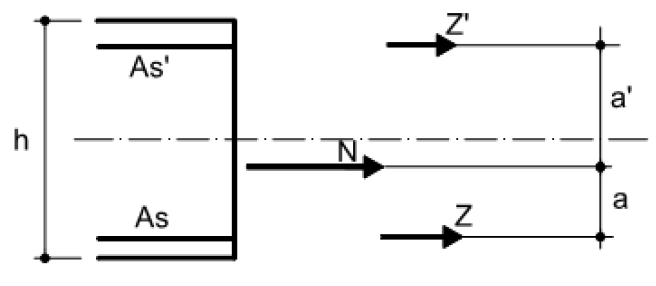
\includegraphics[width=0.8\linewidth]{images/Risse8ZugklEx.PNG}
%\end{minipage}
%\begin{minipage}{0.6\linewidth}
%	
%	falls N innerhalb Bewehrungslagen $ \rightarrow $ Steifigkeit allein durch Stahl bestimmt
%	
%	\begin{tabular}{p{0.3\linewidth}|p{0.3\linewidth}|l}
%		
%		Bemerkung		& Formel		& Einheit \\ \hline
%		
%		
%		Steifigkeit		& $ EI = E_{s} \cdot I_s = EI^{II} $	&	\\
%		
%		Spannung		& $ \sigma_s = \frac{N}{A_s} \frac{a'}{a + a'} $		& $ \left[ \frac{kN}{mm^2}\right] $ \\	
%		
%		& $ \sigma'_s = \frac{N}{A'_s} \frac{a'}{a + a'} $	& $ \left[ \frac{kN}{mm^2}\right] $ \\	
%		
%	\end{tabular}
%\end{minipage}
%
%
%
%\subsubsection{Druck und Zug, grosse Exzentrizität}
%
%\begin{minipage}{0.35\linewidth}
%	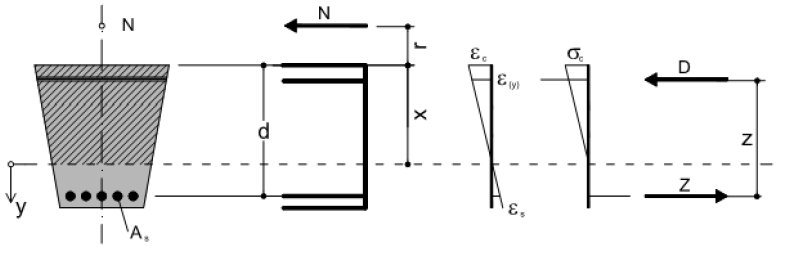
\includegraphics[width=0.9\linewidth]{images/Risse7grEx.PNG}
%\end{minipage}
%\begin{minipage}{0.6\linewidth}
%	
%	Greift N nicht im Kern an, kann die Ausmitte nicht vernachlässigt werden $ \rightarrow $ e>k
%	
%	\begin{tabular}{p{0.3\linewidth}|p{0.45\linewidth}|l}
%		
%		Bemerkung		& Formel		& Einheit \\ \hline
%		
%		
%		Lage der Nullachse & $ r + x = \frac{I_i}{S_i} $	& [mm] \\
%		$ \rightarrow $ Gleich nach x auflösen, so dass S$_i$ = 0	& 	& 	\\		
%		
%		Für Rechteck	& $ r + x = \frac{  \frac{b \cdot x^3}{3}  + n \cdot A_s ( d - x )^2  }{  \frac{b \cdot x^2}{2} - n \cdot A_s ( d -  x )  } $	&	[mm] \\
%		
%		Spannung		& $ \sigma_c = \varepsilon_c \cdot E_c = \frac{ N ( r + x ) }{I_i} \cdot x $	& $ \left[ \frac{kN}{mm^2}\right] $ \\
%						& $ \sigma_s = \varepsilon_s \cdot E_s = n \cdot \frac{ N ( r + x ) }{I_i} \cdot (d - x) $	& $ \left[ \frac{kN}{mm^2}\right] $ \\	
%		Steifigkeit		& $ EI = E_{cm} \cdot I_i = EI^{II} $	&	\\
%				
%	\end{tabular}
%\end{minipage}

\clearpage

\begin{multicols}{2}
	
	
	\subsection{Biegung mit Normalkraft}
	
	
	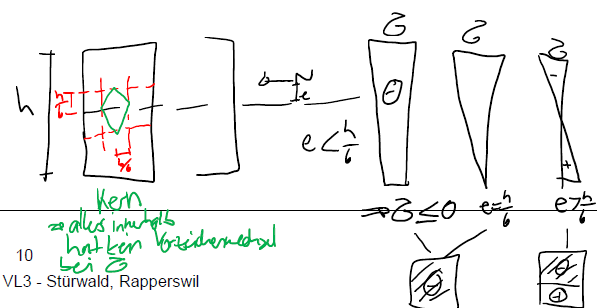
\includegraphics[width=\linewidth]{images/Risse6Kern.PNG}
	
	
	Kernweiten:	 $ k_{1/2} = \frac{I_i}{A_i \cdot y_{2/1}} = \frac{W_y}{A} = \frac{  \frac{b \cdot h^2}{6}  }{b \cdot h} $  [m] \\	
	Exzentrizität: $ e = -\frac{M}{N} $ [mm]
	
	
	
	\subsubsection{Druck, kleine Exzentrizität}
	
	
	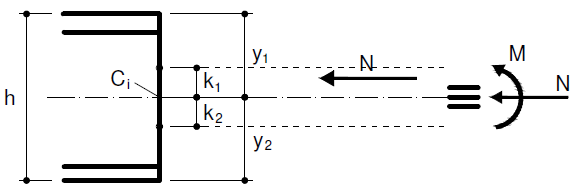
\includegraphics[width=0.7\linewidth]{images/Risse5klExPNG} \\
	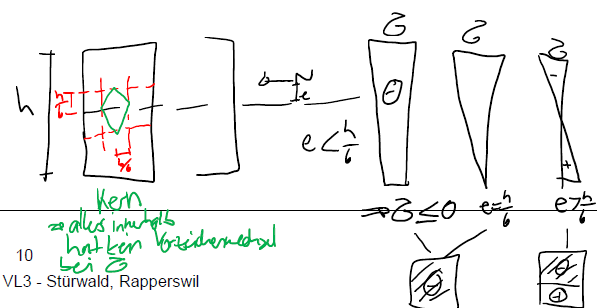
\includegraphics[width=\linewidth]{images/Risse6Kern.PNG}
	
	
	Greift N im Kern an, kann die Ausmitte vernachlässigt werden $ \rightarrow $ zentrischer Druck
	
	\begin{tabular}{p{0.3\linewidth}|p{0.3\linewidth}|l}
		
		Bemerkung		& Formel		& Einheit \\ \hline
		
		
		Spannung		& $ \sigma_c = \varepsilon_c \cdot E_c = \frac{N}{A_i} \pm \frac{M}{I_i}y $	& $ \left[ \frac{kN}{mm^2} \right]$ \\
		& $ \sigma_s = \varepsilon_s \cdot E_s = n \cdot \sigma_c $	& $ \left[ \frac{kN}{mm^2} \right]$ \\
		
		Steifigkeit	& $ EI = E_{cm} \cdot I_i = EI^1 $	& \\
		
	\end{tabular}
	
	
	\subsubsection{Zug mit kleiner Ausmitte}

	
		
	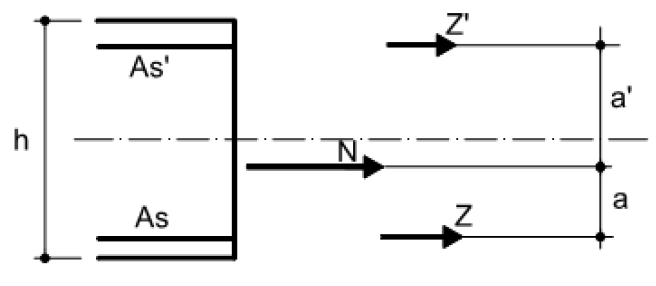
\includegraphics[width=0.5\linewidth]{images/Risse8ZugklEx.PNG}
	
	
	falls N innerhalb Bewehrungslagen $ \rightarrow $ Steifigkeit allein durch Stahl bestimmt
	
	\begin{tabular}{p{0.3\linewidth}|p{0.3\linewidth}|l}
		
		Bemerkung		& Formel		& Einheit \\ \hline
		
		
		Steifigkeit		& $ EI = E_{s} \cdot I_s = EI^{II} $	&	\\
		
		Spannung		& $ \sigma_s = \frac{N}{A_s} \frac{a'}{a + a'} $		& $ \left[ \frac{kN}{mm^2}\right] $ \\	
		
		& $ \sigma'_s = \frac{N}{A'_s} \frac{a'}{a + a'} $	& $ \left[ \frac{kN}{mm^2}\right] $ 
	
	\end{tabular}
	
	
	
	\subsubsection{Druck und Zug, grosse Exzentrizität}
	
	
	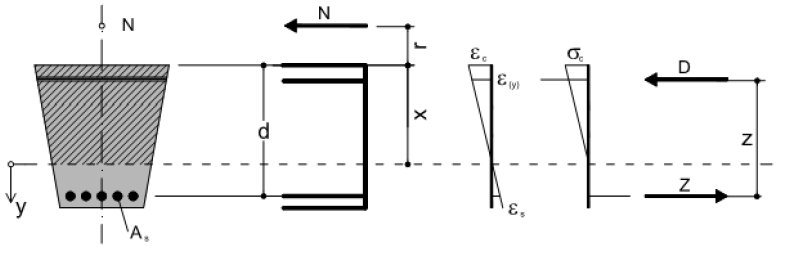
\includegraphics[width=\linewidth]{images/Risse7grEx.PNG}
	
	Greift N nicht im Kern an, kann die Ausmitte nicht vernachlässigt werden $ \rightarrow $ e>k
	
	\begin{tabular}{p{0.3\linewidth}|p{0.5\linewidth}|l}
		
		Bemerkung		& Formel		& Einheit \\ \hline
		
		
		Lage der Nullachse & $ r + x = \frac{I_i}{S_i} $	& [mm] \\
			&  $ \rightarrow $ Gleich nach x auflösen, so dass S$_i$ = 0	& 	\\		
		
		Für Rechteck	& $ r + x = \frac{  \frac{b \cdot x^3}{3}  + n \cdot A_s ( d - x )^2  }{  \frac{b \cdot x^2}{2} - n \cdot A_s ( d -  x )  } $	&	[mm] \\
		
		Spannung		& $ \sigma_c = \varepsilon_c \cdot E_c = \frac{ N ( r + x ) }{I_i} \cdot x $	& $ \left[ \frac{kN}{mm^2}\right] $ \\
		& $ \sigma_s = \varepsilon_s \cdot E_s = n \cdot \frac{ N ( r + x ) }{I_i} \cdot (d - x) $	& $ \left[ \frac{kN}{mm^2}\right] $ \\	
		Steifigkeit		& $ EI = E_{cm} \cdot I_i = EI^{II} $	&	\\
		
	\end{tabular}
	
	
\end{multicols}